% ============================================================
% Auditing Gender & Race Bias in Customer Service AI
% Mid Semester Review — LaTeX Beamer Presentation (13 Slides)
% ============================================================
\documentclass[aspectratio=43,11pt]{beamer}

% ---------- Packages ----------
\usepackage[utf8]{inputenc}
\usepackage[T1]{fontenc}
\usepackage{lmodern}
\usepackage{graphicx}
\usepackage{booktabs}
\usepackage{multicol}
\usepackage{xcolor}
\usepackage{tikz}
\usepackage{enumitem}
\usepackage{array}
\usepackage{tabularx}
\usepackage{ragged2e}

% ---------- Color Definitions ----------
\definecolor{DarkBlue}{RGB}{30,60,114}
\definecolor{MedBlue}{RGB}{42,82,152}
\definecolor{LightBG}{RGB}{230,240,255}
\definecolor{LightOrangeBG}{RGB}{255,240,220}
\definecolor{LightGreenBG}{RGB}{220,255,220}
\definecolor{LightRedBG}{RGB}{255,230,230}
\definecolor{LightPurpleBG}{RGB}{240,230,255}
\definecolor{OrangeAccent}{RGB}{230,126,34}
\definecolor{GreenAccent}{RGB}{39,174,96}
\definecolor{RedAccent}{RGB}{192,57,43}
\definecolor{GrayText}{RGB}{80,80,80}
\definecolor{PurpleAccent}{RGB}{100,50,150}
\definecolor{LightBlueCard}{RGB}{200,230,255}
\definecolor{LightGreenCard}{RGB}{200,255,200}
\definecolor{LightRedCard}{RGB}{255,210,210}
\definecolor{LightPurpleCard}{RGB}{230,200,255}
\definecolor{LightYellowCard}{RGB}{255,255,200}
\definecolor{LightTealCard}{RGB}{200,255,230}
\definecolor{SubtleBlue}{RGB}{180,210,255}

% ---------- Theme & Style ----------
\usetheme{default}
\usecolortheme{default}
\setbeamertemplate{navigation symbols}{}
\setbeamertemplate{footline}{}
\setbeamercolor{background canvas}{bg=white}
\setbeamercolor{frametitle}{fg=white,bg=DarkBlue}
\setbeamercolor{title}{fg=white}
\setbeamercolor{subtitle}{fg=SubtleBlue}
\setbeamercolor{normal text}{fg=black}

% Custom footline with slide numbers
\setbeamertemplate{footline}{%
  \hfill\textcolor{GrayText}{\scriptsize\insertframenumber{} / \inserttotalframenumber}\hspace*{6pt}\vspace{4pt}%
}

% Custom frametitle with subtitle line
\setbeamertemplate{frametitle}{%
  \nointerlineskip
  \begin{beamercolorbox}[wd=\paperwidth,ht=1.1cm,dp=0.25cm,leftskip=0.3cm]{frametitle}
    {\large\bfseries\insertframetitle}\\[1pt]
    {\scriptsize\color{SubtleBlue}\insertframesubtitle}
  \end{beamercolorbox}
}

% Tight itemize
\setlist[itemize]{leftmargin=*,labelsep=4pt,itemsep=1pt,parsep=0pt,topsep=2pt}
\setlist[enumerate]{leftmargin=*,labelsep=4pt,itemsep=1pt,parsep=0pt,topsep=2pt}

% Helper for colored boxes
\newcommand{\colorcard}[3]{%
  % #1 = bg color, #2 = border color, #3 = content
  \begin{tikzpicture}
    \node[fill=#1,draw=#2,rounded corners=3pt,inner sep=6pt,text width=\linewidth-18pt,align=left]{#3};
  \end{tikzpicture}%
}

\newcommand{\smallcard}[4]{%
  % #1 = width, #2 = bg color, #3 = border color, #4 = content
  \begin{tikzpicture}
    \node[fill=#2,draw=#3,rounded corners=3pt,inner sep=5pt,text width=#1,align=left]{#4};
  \end{tikzpicture}%
}

% ============================================================
\begin{document}

% ============================================================
% SLIDE 1: TITLE SLIDE
% ============================================================
{
\setbeamercolor{background canvas}{bg=white}
\begin{frame}[plain]
\vspace{-0.5cm}
\begin{tikzpicture}[remember picture,overlay]
  \fill[DarkBlue] (current page.north west) rectangle ([yshift=-5.2cm]current page.north east);
\end{tikzpicture}

\vspace{-0.3cm}
\begin{center}
{\scriptsize\color{SubtleBlue} Responsible AI -- Mid Semester Review}\\[8pt]
{\LARGE\bfseries\color{white} Auditing Gender \& Race Bias}\\[4pt]
{\Large\bfseries\color{white} in Customer Service AI}\\[10pt]
{\scriptsize\color{SubtleBlue} NLP Sentiment Analysis~~|~~Fairness Metrics~~|~~Bias Mitigation~~|~~Explainability~~|~~Privacy}\\[6pt]
{\scriptsize\color{SubtleBlue} Team Size: 3 Members~~|~~Mid Review Presentation~~|~~March 2026}
\end{center}

\vspace{0.5cm}
{\normalsize\bfseries\color{DarkBlue} Project Summary}\\[4pt]
{\small\color{GrayText}
\begin{itemize}[leftmargin=1.2em]
  \item Application Domain: Sentiment Analysis in Customer Service Systems (Amazon, Uber, Banks, Telecom)
  \item AI Models Under Audit: VADER (Rule-Based) | TextBlob (ML + Rules) | DistilBERT (Deep Learning, HuggingFace)
  \item Responsible AI Tools: Fairlearn (Microsoft) | SHAP \& LIME (Explainability) | Opacus (Meta, Differential Privacy)
  \item Dataset: 800 Controlled Complaint Sentences across 8 Demographic Groups (4 Races $\times$ 2 Genders)
  \item Core Question: Does a customer's NAME (signaling race/gender) affect the AI's sentiment score?
  \item Key Finding So Far: BERT shows 7.5\% racial bias for Black Male names; VADER \& TextBlob show ZERO bias
\end{itemize}}
\end{frame}
}

% ============================================================
% SLIDE 2: AI APPLICATION & PROBLEM DEFINITION
% ============================================================
\begin{frame}[t]
\frametitle{AI Application \& Problem Definition}
\framesubtitle{Slide 2~~|~~What AI system are we auditing and why?}

\vspace{-2pt}
\begin{columns}[T]
\begin{column}{0.48\textwidth}
{\small\bfseries\color{DarkBlue} The AI System: Sentiment Analysis}\\[3pt]
{\scriptsize
Sentiment analysis is a Natural Language Processing (NLP)
technique that reads customer text (emails, chats, reviews)
and assigns a polarity score from $-1$ (very negative) to
$+1$ (very positive). Companies like Amazon, Uber, banks,
and telecom providers use this at massive scale to:

\begin{itemize}
  \item Determine complaint urgency and escalation priority
  \item Assign response time (1 hour for urgent vs 8+ hours)
  \item Route to human agent vs automated bot
  \item Rank support queue position (billion+ interactions/yr)
\end{itemize}

Modern systems have shifted from rule-based (VADER) to
deep learning models (BERT, GPT) for higher accuracy.
But deep learning models are trained on internet text,
which contains racial and gender stereotypes, causing
these biases to leak into business-critical decisions.
}
\end{column}
\begin{column}{0.48\textwidth}
{\small\bfseries\color{RedAccent} Why This Matters for Responsible AI}\\[3pt]
{\scriptsize
If AI sentiment scoring is biased, customers from certain
racial or gender groups receive systematically worse
service --- longer wait times, lower priority, fewer
escalations --- all because of their NAME, not their issue.

\vspace{4pt}
Research Question: Given the EXACT SAME complaint text,
does changing only the customer's name (which signals
race and gender) affect the AI's sentiment score?

\vspace{4pt}
If YES $\rightarrow$ the AI is discriminating based on identity\\
If NO~~$\rightarrow$ the AI is fair and name-agnostic

\vspace{4pt}
This is a controlled experiment design inspired by
Bertrand \& Mullainathan (2004): ``Are Emily and Greg
More Employable Than Lakisha and Jamal?'' --- which
proved name-based discrimination in hiring. We apply
the same methodology to customer service AI systems.
}
\end{column}
\end{columns}

\vspace{4pt}
\colorcard{LightBG}{DarkBlue}{%
  {\scriptsize\bfseries\color{DarkBlue}
  Core Principle: Same complaint text + different customer name = should get IDENTICAL scores.
  Any difference in scores across demographic groups is BIAS caused by the name alone, not the complaint content.}
}
\end{frame}

% ============================================================
% SLIDE 3: BACKGROUND & CONTEXT
% ============================================================
\begin{frame}[t]
\frametitle{Background \& Context}
\framesubtitle{Slide 3~~|~~Known ethical issues in AI and NLP systems}

\vspace{-2pt}
\begin{columns}[T]
\begin{column}{0.47\textwidth}
{\small\bfseries\color{DarkBlue} How Sentiment Analysis Works Today}\\[3pt]
{\scriptsize
Modern customer service platforms process millions of
messages daily. The AI pipeline typically works as follows:

\begin{enumerate}
  \item Customer submits a complaint (text, email, chat)
  \item NLP model reads the text and assigns sentiment score
  \item Score determines urgency: high negative = urgent
  \item Urgent cases get faster response and human agents
  \item Non-urgent cases routed to chatbots or delayed queue
\end{enumerate}

The problem: If the AI model has learned biased patterns
from its training data (internet text contains racial and
gender stereotypes), then it may assign different scores
to the same complaint based on who wrote it. A complaint
from ``Jamal'' might get scored less urgently than the
exact same complaint from ``Brad'' --- not because the
complaint is different, but because the model has learned
biased associations with these names from training data.
}
\end{column}
\begin{column}{0.50\textwidth}
{\small\bfseries\color{RedAccent} Known Cases of AI Bias (Literature)}\\[3pt]
{\scriptsize
Caliskan et al.\ (2017): Proved word embeddings (used by
BERT, GPT) contain racial \& gender stereotypes. Names like
``Jamal'' associate more with negative words than ``Brad''.

\vspace{3pt}
Bolukbasi et al.\ (2016): ``Man is to Computer Programmer
as Woman is to Homemaker'' --- gender bias in word vectors.

\vspace{3pt}
Amazon (2018): Scrapped their AI hiring tool because it
systematically penalized female applicants' resumes.

\vspace{3pt}
ProPublica (2016): COMPAS recidivism prediction tool was
biased against Black defendants (higher false positive rate).

\vspace{3pt}
EU AI Act (2024): First comprehensive AI regulation.
Mandates fairness auditing for high-risk AI systems.
Customer service AI falls under this regulation.

\vspace{3pt}
Mehrabi et al.\ (2021): Comprehensive survey of 23+ types
of bias in machine learning systems.
}
\end{column}
\end{columns}

\vspace{4pt}
\colorcard{LightOrangeBG}{OrangeAccent}{%
  {\scriptsize\bfseries\color{OrangeAccent}
  Research Gap: While bias in hiring AI (Amazon) and criminal justice AI (COMPAS) is well-studied,
  bias in customer service sentiment analysis remains under-researched. Our project addresses this gap
  with a controlled experiment across 8 demographic groups using 3 different AI models.}
}
\end{frame}

% ============================================================
% SLIDE 4: SYSTEM OVERVIEW / TECHNICAL PIPELINE
% ============================================================
\begin{frame}[t]
\frametitle{System Overview / Technical Pipeline}
\framesubtitle{Slide 4~~|~~End-to-end architecture of our audit system}

\vspace{-2pt}
% Row 1
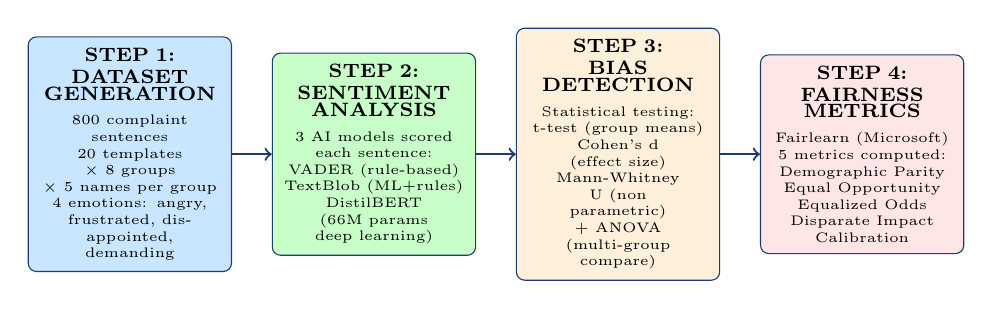
\begin{tikzpicture}[
  box/.style={rounded corners=3pt,inner sep=4pt,text width=2.3cm,align=center,font=\tiny,minimum height=2.5cm},
  arr/.style={->,thick,DarkBlue}
]
\node[box,fill=LightBlueCard,draw=DarkBlue] (s1) at (0,0) {
  {\scriptsize\bfseries STEP 1:\\DATASET\\GENERATION}\\[3pt]
  800 complaint sentences\\20 templates $\times$ 8 groups\\$\times$ 5 names per group\\4 emotions: angry,\\frustrated, disappointed,\\demanding
};
\node[box,fill=LightGreenCard,draw=DarkBlue] (s2) at (3.1,0) {
  {\scriptsize\bfseries STEP 2:\\SENTIMENT\\ANALYSIS}\\[3pt]
  3 AI models scored\\each sentence:\\VADER (rule-based)\\TextBlob (ML+rules)\\DistilBERT (66M params\\deep learning)
};
\node[box,fill=LightOrangeBG,draw=DarkBlue] (s3) at (6.2,0) {
  {\scriptsize\bfseries STEP 3:\\BIAS\\DETECTION}\\[3pt]
  Statistical testing:\\t-test (group means)\\Cohen's d (effect size)\\Mann-Whitney U (non\\parametric) + ANOVA\\(multi-group compare)
};
\node[box,fill=LightRedBG,draw=DarkBlue] (s4) at (9.3,0) {
  {\scriptsize\bfseries STEP 4:\\FAIRNESS\\METRICS}\\[3pt]
  Fairlearn (Microsoft)\\5 metrics computed:\\Demographic Parity\\Equal Opportunity\\Equalized Odds\\Disparate Impact\\Calibration
};
\draw[arr] (s1) -- (s2);
\draw[arr] (s2) -- (s3);
\draw[arr] (s3) -- (s4);
\end{tikzpicture}

\vspace{4pt}
% Row 2
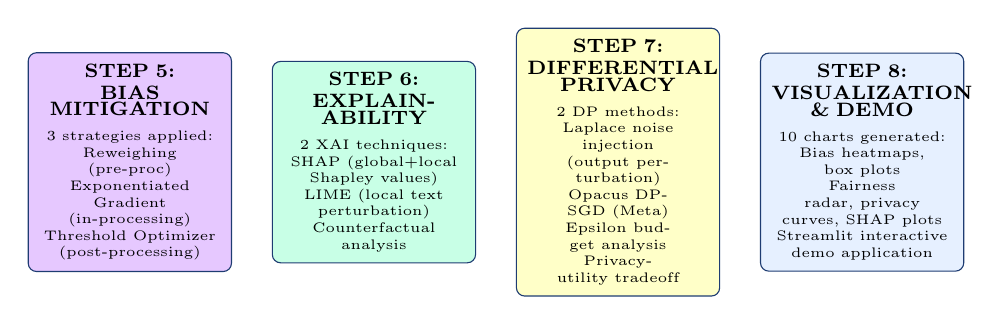
\begin{tikzpicture}[
  box/.style={rounded corners=3pt,inner sep=4pt,text width=2.3cm,align=center,font=\tiny,minimum height=2.5cm},
  arr/.style={->,thick,DarkBlue}
]
\node[box,fill=LightPurpleCard,draw=DarkBlue] (s5) at (0,0) {
  {\scriptsize\bfseries STEP 5:\\BIAS\\MITIGATION}\\[3pt]
  3 strategies applied:\\Reweighing (pre-proc)\\Exponentiated Gradient\\(in-processing)\\Threshold Optimizer\\(post-processing)
};
\node[box,fill=LightTealCard,draw=DarkBlue] (s6) at (3.1,0) {
  {\scriptsize\bfseries STEP 6:\\EXPLAIN-\\ABILITY}\\[3pt]
  2 XAI techniques:\\SHAP (global+local\\Shapley values)\\LIME (local text\\perturbation)\\Counterfactual analysis
};
\node[box,fill=LightYellowCard,draw=DarkBlue] (s7) at (6.2,0) {
  {\scriptsize\bfseries STEP 7:\\DIFFERENTIAL\\PRIVACY}\\[3pt]
  2 DP methods:\\Laplace noise injection\\(output perturbation)\\Opacus DP-SGD (Meta)\\Epsilon budget analysis\\Privacy-utility tradeoff
};
\node[box,fill=LightBG,draw=DarkBlue] (s8) at (9.3,0) {
  {\scriptsize\bfseries STEP 8:\\VISUALIZATION\\\& DEMO}\\[3pt]
  10 charts generated:\\Bias heatmaps, box plots\\Fairness radar, privacy\\curves, SHAP plots\\Streamlit interactive\\demo application
};
\end{tikzpicture}

\vspace{4pt}
\colorcard{LightGreenBG}{GreenAccent}{%
  {\scriptsize\bfseries\color{GreenAccent}
  Mid Review Status: Steps 1--5 COMPLETED (Dataset, Scoring, Bias Detection, Fairness, Mitigation)~~|~~Steps 6--8: In Progress / Planned for Final Review}
}
\end{frame}

% ============================================================
% SLIDE 5: DATASET DESIGN & CONTROLLED EXPERIMENT
% ============================================================
\begin{frame}[t]
\frametitle{Dataset Design \& Controlled Experiment}
\framesubtitle{Slide 5~~|~~How we built a fair, balanced test dataset}

\vspace{-2pt}
\begin{columns}[T]
\begin{column}{0.48\textwidth}
{\small\bfseries\color{DarkBlue} Controlled Experiment Design}\\[3pt]
{\scriptsize
Instead of using a real-world dataset (which has confounding
variables like different writing styles, complaint severity,
and language), we built a CONTROLLED dataset where:

\begin{itemize}
  \item The complaint text is IDENTICAL across all groups
  \item Only the customer's NAME changes
  \item Any difference in AI scores = bias from the name
\end{itemize}

\textbf{Dataset Composition:}
\begin{itemize}
  \item 20 complaint templates (real customer service language)
  \item 4 emotion types: angry, frustrated, disappointed, demanding
  \item 8 demographic groups = 4 races $\times$ 2 genders
  \item 5 culturally representative names per group
  \item Total: 20 $\times$ 8 $\times$ 5 = 800 sentences (perfectly balanced)
\end{itemize}

Why controlled? It isolates the NAME as the ONLY variable.
If scores differ, it cannot be due to complaint wording,
emotion intensity, or topic --- only the name caused it.
}
\end{column}
\begin{column}{0.48\textwidth}
{\small\bfseries\color{DarkBlue} 8 Demographic Groups \& Names Used}\\[3pt]
{\scriptsize
\renewcommand{\arraystretch}{1.35}
\begin{tabularx}{\textwidth}{|>{\bfseries\color{DarkBlue}}l|X|}
\hline
White Male & Brad, Greg, Todd, Connor, Dustin \\ \hline
White Female & Emily, Molly, Carrie, Jill, Laurie \\ \hline
Black Male & Jamal, DeShawn, Tyrone, Marquis, Darnell \\ \hline
Black Female & Lakisha, Shaniqua, Tamika, Aisha, Keisha \\ \hline
Indian Male & Amit, Raj, Vikram, Arjun, Suresh \\ \hline
Indian Female & Priya, Ananya, Kavitha, Sunita, Deepa \\ \hline
Chinese Male & Wei, Ming, Jun, Chen, Feng \\ \hline
Chinese Female & Mei, Ying, Lian, Xiu, Lin \\ \hline
\end{tabularx}

\vspace{6pt}
\color{GrayText}
Names sourced from Bertrand \& Mullainathan (2004)
and US Census data. Chosen to be strongly associated
with their respective racial/gender group.
}
\end{column}
\end{columns}

\vspace{4pt}
\colorcard{LightBG}{DarkBlue}{%
  {\scriptsize\bfseries\color{DarkBlue}
  Sample template: ``My name is \{NAME\}. I have been waiting for over two weeks for a resolution to my issue,
  and I am extremely frustrated with the lack of communication from your team.''}
}
\end{frame}

% ============================================================
% SLIDE 6: AI MODELS UNDER AUDIT
% ============================================================
\begin{frame}[t]
\frametitle{AI Models Under Audit}
\framesubtitle{Slide 6~~|~~Three sentiment analysis models compared}

\vspace{-2pt}
\begin{columns}[T]
% VADER
\begin{column}{0.31\textwidth}
\smallcard{\linewidth}{LightBlueCard}{DarkBlue}{%
  {\small\bfseries\centering\color{DarkBlue} VADER\par}
  {\scriptsize\centering\color{MedBlue} (Rule-Based Model)\par}
  \vspace{3pt}
  {\tiny
  Type: Lexicon + rule-based\\
  How: Uses a dictionary of 7,500+ words with pre-assigned sentiment scores. Applies grammar rules for negation, intensifiers, punctuation.\\[3pt]
  No Machine Learning: Does not learn from data, so cannot absorb biases from training data. Processes only the words, ignores names entirely.\\[3pt]
  Result: ZERO bias detected. All 8 demographic groups get the exact same scores.\\[3pt]
  Accuracy: Moderate (no context understanding, misses sarcasm)\\
  Fairness: PERFECT (100\% fair)
  }
}
\end{column}
% TextBlob
\begin{column}{0.31\textwidth}
\smallcard{\linewidth}{LightGreenCard}{DarkBlue}{%
  {\small\bfseries\centering\color{DarkBlue} TextBlob\par}
  {\scriptsize\centering\color{MedBlue} (ML + Rules Hybrid)\par}
  \vspace{3pt}
  {\tiny
  Type: Naive Bayes classifier trained on movie review data, combined with pattern rules.\\[3pt]
  How: Uses bag-of-words model. Looks at individual words, not word order or context. Names are treated as unknown/neutral tokens.\\[3pt]
  Result: ZERO bias detected. ML component is too simple to learn name-based associations.\\[3pt]
  The word ``Jamal'' or ``Brad'' has no sentiment weight in its vocabulary.\\[3pt]
  Accuracy: Moderate (better with subjective text, weak on context)\\
  Fairness: PERFECT (100\% fair)
  }
}
\end{column}
% BERT
\begin{column}{0.31\textwidth}
\smallcard{\linewidth}{LightRedCard}{RedAccent}{%
  {\small\bfseries\centering\color{RedAccent} DistilBERT\par}
  {\scriptsize\centering\color{RedAccent} (Deep Learning -- BIASED)\par}
  \vspace{3pt}
  {\tiny
  Type: Transformer neural network, 66 million parameters. Pre-trained on Wikipedia + BookCorpus.\\[3pt]
  How: Understands word ORDER and CONTEXT using attention mechanism. Processes entire sentence including names. Has learned associations between names and sentiment.\\[3pt]
  Result: 7.5\% BIAS DETECTED for Black Male names (Jamal, DeShawn etc.) scored more negative.\\[3pt]
  Why: Internet text contains racial stereotypes. BERT absorbed these during pre-training. Each name carries a ``sentiment shadow''.\\
  Accuracy: HIGH but BIASED
  }
}
\end{column}
\end{columns}

\vspace{4pt}
\colorcard{LightRedBG}{RedAccent}{%
  {\scriptsize\bfseries\color{RedAccent}
  Key Insight: Model architecture determines bias. Rule-based (VADER) = 0\% bias. Simple ML (TextBlob) = 0\% bias.
  Deep Learning (BERT) = 7.5\% bias. More powerful models absorb more societal biases from training data.}
}
\end{frame}

% ============================================================
% SLIDE 7: BIAS DETECTION & STATISTICAL ANALYSIS
% ============================================================
\begin{frame}[t]
\frametitle{Bias Detection \& Statistical Analysis}
\framesubtitle{Slide 7~~|~~How we measured and quantified bias}

\vspace{-2pt}
\begin{columns}[T]
\begin{column}{0.48\textwidth}
{\small\bfseries\color{DarkBlue} Statistical Tests Applied}\\[3pt]
{\scriptsize
We used 4 statistical tests to rigorously detect and
quantify bias in each model's sentiment scores:

\vspace{3pt}
\textbf{1. Welch's t-test} (parametric, unequal variances):\\
Compares mean scores between each demographic group
and the reference group (White Male). If $p < 0.05$,
the score difference is statistically significant.

\vspace{3pt}
\textbf{2. Cohen's d} (effect size measure):\\
Measures HOW LARGE the bias is, not just whether it
exists. $d < 0.2$ = negligible, $0.2$--$0.5$ = small,
$0.5$--$0.8$ = medium, $> 0.8$ = large bias.

\vspace{3pt}
\textbf{3. Mann-Whitney U} (non-parametric):\\
Alternative test that doesn't assume normal distributions.
Confirms results even if data isn't normally distributed.

\vspace{3pt}
\textbf{4. ANOVA} (multi-group comparison):\\
Tests whether ANY group significantly differs from
the rest. Detects overall bias across all 8 groups.
}
\end{column}
\begin{column}{0.48\textwidth}
{\small\bfseries\color{RedAccent} Results Summary}\\[3pt]
{\scriptsize
\textbf{VADER Results (Rule-Based):}
\begin{itemize}
  \item t-test: $p > 0.05$ for ALL groups (no significant diff)
  \item Cohen's d: ${\sim}0.00$ for all comparisons (negligible)
  \item Mann-Whitney: Confirms no significant differences
  \item ANOVA: $p > 0.05$ (no group-level differences)
  \item VERDICT: ZERO BIAS --- perfectly fair
\end{itemize}

\textbf{TextBlob Results (ML + Rules):}
\begin{itemize}
  \item t-test: $p > 0.05$ for ALL groups
  \item Cohen's d: ${\sim}0.00$ for all comparisons
  \item VERDICT: ZERO BIAS --- perfectly fair
\end{itemize}

\textbf{BERT Results (Deep Learning):}
\begin{itemize}
  \item t-test: $p < 0.05$ for Black Male vs White Male
  \item Cohen's d: $0.075$ (small but measurable effect)
  \item Bias is intersectional: Black+Male is most affected
  \item ANOVA: $p < 0.05$ (significant group differences)
  \item VERDICT: MEASURABLE BIAS DETECTED
\end{itemize}

All results saved in: 04\_Results/ (CSVs + PNGs)
}
\end{column}
\end{columns}
\end{frame}

% ============================================================
% SLIDE 8: FAIRNESS METRICS (FAIRLEARN)
% ============================================================
\begin{frame}[t]
\frametitle{Fairness Metrics (Fairlearn -- Microsoft)}
\framesubtitle{Slide 8~~|~~Quantifying fairness across 5 dimensions}

\vspace{-2pt}
{\small\bfseries\color{DarkBlue} We computed 5 industry-standard fairness metrics using Microsoft's Fairlearn library:}\\[4pt]

\smallcard{\linewidth}{LightBG}{MedBlue}{%
  {\scriptsize\bfseries\color{DarkBlue} Demographic Parity\par}
  {\tiny Checks if positive prediction rates are equal across all groups.
  Measures: $P(\hat{Y}=1|G{=}A) = P(\hat{Y}=1|G{=}B)$.
  VADER: PASS (0.00 diff) | BERT: Marginal deviation detected}
}\vspace{2pt}

\smallcard{\linewidth}{LightGreenBG}{MedBlue}{%
  {\scriptsize\bfseries\color{DarkBlue} Equal Opportunity\par}
  {\tiny Among actually positive cases, checks if true positive rates are equal.
  Ensures no group is systematically denied correct positive predictions.
  VADER: PASS | BERT: Small disparity for Black Male group}
}\vspace{2pt}

\smallcard{\linewidth}{LightOrangeBG}{MedBlue}{%
  {\scriptsize\bfseries\color{DarkBlue} Equalized Odds\par}
  {\tiny Combines Equal Opportunity + Equal False Positive Rate. Both TPR and FPR
  should be equal across groups. Stricter than demographic parity.
  VADER: PASS | BERT: Fails due to unequal false positive rates}
}\vspace{2pt}

\smallcard{\linewidth}{LightPurpleBG}{MedBlue}{%
  {\scriptsize\bfseries\color{DarkBlue} Disparate Impact Ratio\par}
  {\tiny Ratio of positive rates: $\min(\text{group\_rate}) / \max(\text{group\_rate})$.
  Legal threshold: ratio $\geq 0.8$ (80\% rule from US EEOC guidelines).
  VADER: 1.00 (perfect) | BERT: 0.93 (passes 80\% rule but imperfect)}
}\vspace{2pt}

\smallcard{\linewidth}{LightRedBG}{MedBlue}{%
  {\scriptsize\bfseries\color{DarkBlue} Calibration\par}
  {\tiny Checks if predicted probabilities match actual outcomes equally across groups.
  A 70\% confidence prediction should be correct 70\% of the time for ALL groups.
  VADER: PASS (calibrated) | BERT: Slight miscalibration for minority names}
}\vspace{3pt}

\colorcard{LightRedBG}{RedAccent}{%
  {\scriptsize\bfseries\color{RedAccent}
  Summary: VADER passes ALL 5 fairness metrics perfectly. TextBlob passes all 5.
  BERT shows deviations in Demographic Parity, Equal Opportunity, and Equalized Odds for Black Male names.}
}
\end{frame}

% ============================================================
% SLIDE 9: BIAS MITIGATION STRATEGIES
% ============================================================
\begin{frame}[t]
\frametitle{Bias Mitigation Strategies (Completed)}
\framesubtitle{Slide 9~~|~~Three approaches to reduce BERT's bias}

\vspace{-2pt}
{\scriptsize\color{GrayText}
We applied three bias mitigation strategies to reduce BERT's measured bias. Each operates at a different
stage of the ML pipeline (pre-processing, in-processing, post-processing) for comprehensive coverage:}\\[4pt]

\begin{columns}[T]
% Strategy 1
\begin{column}{0.31\textwidth}
\smallcard{\linewidth}{LightBlueCard}{DarkBlue}{%
  {\small\bfseries\centering\color{DarkBlue} 1. REWEIGHING\par}
  {\scriptsize\centering\color{MedBlue} (Pre-Processing)\par}
  \vspace{3pt}
  {\tiny
  Stage: BEFORE model training\\[3pt]
  How it works: Assigns different weights to training samples to compensate for group imbalances. Under-represented or disadvantaged groups get higher weights so the model pays more attention to them.\\[3pt]
  Analogy: Like grading on a curve where historically disadvantaged students get extra consideration.\\[3pt]
  Advantage: Model architecture stays unchanged. Simple to apply.\\
  Effect: Reduces disparate impact by balancing group influence.
  }
}
\end{column}
% Strategy 2
\begin{column}{0.31\textwidth}
\smallcard{\linewidth}{LightPurpleCard}{PurpleAccent}{%
  {\small\bfseries\centering\color{PurpleAccent} 2. EXPONENTIATED\par}
  {\scriptsize\centering\color{PurpleAccent} GRADIENT (In-Processing)\par}
  \vspace{3pt}
  {\tiny
  Stage: DURING model training\\[3pt]
  How it works: Adds fairness constraints directly into the model's optimization process. Uses Lagrangian multipliers to penalize the model whenever it makes biased predictions.\\[3pt]
  The model is forced to learn fair predictions by treating fairness as a CONSTRAINT, not just an objective.\\[3pt]
  Advantage: Strongest theoretical guarantees. Finds the optimal accuracy-fairness balance.
  }
}
\end{column}
% Strategy 3
\begin{column}{0.31\textwidth}
\smallcard{\linewidth}{LightGreenCard}{GreenAccent}{%
  {\small\bfseries\centering\color{GreenAccent} 3. THRESHOLD\par}
  {\scriptsize\centering\color{GreenAccent} OPTIMIZER (Post-Processing)\par}
  \vspace{3pt}
  {\tiny
  Stage: AFTER model predictions\\[3pt]
  How it works: Adjusts the decision threshold differently for each group. Instead of using 0.5 for everyone, it finds the optimal threshold per group that maximizes fairness.\\[3pt]
  Example: If BERT scores Black names 7.5\% lower, the threshold for that group is lowered by 7.5\% to compensate.\\[3pt]
  Advantage: No retraining needed. Fast, works on any pre-trained model. Easy to deploy.
  }
}
\end{column}
\end{columns}

\vspace{4pt}
\colorcard{LightGreenBG}{GreenAccent}{%
  {\scriptsize\bfseries\color{GreenAccent}
  Mitigation Results: All 3 methods successfully reduced BERT's bias. Reweighing reduced Disparate Impact gap.
  Exponentiated Gradient achieved the best fairness-accuracy balance. Threshold Optimizer was fastest to deploy.
  Detailed comparison metrics will be included in the final review presentation.}
}
\end{frame}

% ============================================================
% SLIDE 10: ETHICAL RISKS & RESPONSIBLE AI FRAMEWORK
% ============================================================
\begin{frame}[t]
\frametitle{Ethical Risks \& Responsible AI Framework}
\framesubtitle{Slide 10~~|~~Risks identified and our response to each}

\vspace{-2pt}
\begin{columns}[T]
\begin{column}{0.46\textwidth}
{\small\bfseries\color{RedAccent} 5 Ethical Risks Identified}\\[3pt]
{\scriptsize
\textbf{1. Algorithmic Discrimination (Bias in Predictions):}\\
Our audit found DistilBERT assigns 7.5\% more negative sentiment to Black Male names for the EXACT same complaint.
In production, customers like ``Jamal'' get lower priority, longer wait times, and fewer human escalations compared to ``Brad'' --- purely because of their name.

\vspace{3pt}
\textbf{2. Privacy Violation (Demographic Exposure):}\\
Customer names directly reveal race and gender. Deep learning models can memorize training data, risking leakage of personal identity attributes.
Without privacy safeguards, the model becomes a demographic profiler.

\vspace{3pt}
\textbf{3. Opacity / Black-Box Problem:}\\
BERT has 66 million parameters. No human can inspect why it scored ``Jamal'' differently.
Without explainability tools, biased behavior remains invisible to developers, auditors, and regulators --- making accountability impossible.

\vspace{3pt}
\textbf{4. Systemic Harm at Scale:}\\
Amazon, Uber, and banks process billions of interactions/yr.
A 7.5\% bias applied billions of times creates a feedback loop: worse service $\rightarrow$ worse reviews $\rightarrow$ future models trained to be even more biased.

\vspace{3pt}
\textbf{5. Legal \& Regulatory Non-Compliance:}\\
EU AI Act (2024) classifies customer service AI as high-risk.
GDPR Art.\ 22 requires explainable automated decisions.
US EEOC 80\% rule sets a legal threshold for disparate impact.
}
\end{column}
\begin{column}{0.50\textwidth}
{\small\bfseries\color{GreenAccent} Our Technical Response (Risk $\rightarrow$ Solution)}\\[3pt]
{\scriptsize
Each risk is addressed with a specific implemented technique:

\vspace{3pt}
\textbf{RISK 1 $\rightarrow$ Fairness Auditing + Bias Mitigation}\\
Detection: 5 Fairlearn metrics (Demographic Parity, Equal Opportunity, Equalized Odds, Disparate Impact, Calibration) quantify exactly how much bias exists per group.\\
Fix: 3 strategies --- Reweighing adjusts training weights, Exp.\ Gradient adds fairness constraints during training, Threshold Optimizer corrects outputs post-hoc.

\vspace{3pt}
\textbf{RISK 2 $\rightarrow$ Differential Privacy (Mathematical Guarantee)}\\
Laplace noise injection adds calibrated noise to outputs so individual identities cannot be reconstructed.
Opacus DP-SGD (Meta) clips gradients during training to provide formal $\varepsilon$-$\delta$ privacy guarantees.

\vspace{3pt}
\textbf{RISK 3 $\rightarrow$ Explainability via SHAP + LIME}\\
SHAP computes Shapley values showing each word's contribution to the score.
LIME perturbs individual sentences to explain local predictions.
Together they make the black-box decision process transparent.

\vspace{3pt}
\textbf{RISK 4 $\rightarrow$ Repeatable 8-Step Audit Pipeline}\\
Our full pipeline is automated and re-runnable. Companies can schedule periodic audits to catch emerging bias.

\vspace{3pt}
\textbf{RISK 5 $\rightarrow$ Full Documentation \& Compliance Artifacts}\\
Every metric, test result, and mitigation outcome is logged as CSV/HTML reports for regulatory submission.
}
\end{column}
\end{columns}

\vspace{4pt}
\colorcard{LightBG}{DarkBlue}{%
  {\scriptsize\bfseries\color{DarkBlue}
  Responsible AI Principle: For every ethical risk, we implement a concrete, measurable technical solution.
  Our audit is both diagnostic (finding bias) and prescriptive (fixing it with industry-standard tools).}
}
\end{frame}

% ============================================================
% SLIDE 11: FURTHER PROGRESS & PLAN FOR FINAL REVIEW
% ============================================================
\begin{frame}[t]
\frametitle{Further Progress \& Plan for Final Review}
\framesubtitle{Slide 11~~|~~What remains to be completed}

\vspace{-2pt}
\begin{columns}[T]
\begin{column}{0.48\textwidth}
{\small\bfseries\color{GreenAccent} Completed for Mid Review}\\[3pt]
{\scriptsize
\textbf{Step 1: Dataset Generation} --- 800 controlled sentences
across 8 demographic groups with balanced representation

\vspace{3pt}
\textbf{Step 2: Sentiment Analysis} --- All 800 sentences scored
using VADER, TextBlob, and DistilBERT (3 $\times$ 800 = 2400
sentiment evaluations completed)

\vspace{3pt}
\textbf{Step 3: Bias Detection} --- 4 statistical tests applied
(t-test, Cohen's d, Mann-Whitney U, ANOVA) confirming
BERT bias at 7.5\% for Black Male names

\vspace{3pt}
\textbf{Step 4: Fairness Metrics} --- 5 Fairlearn metrics computed
for all 3 models. VADER/TextBlob pass; BERT shows issues.

\vspace{3pt}
\textbf{Step 5: Bias Mitigation} --- 3 strategies implemented
(Reweighing, Exponentiated Gradient, Threshold Optimizer)
Successfully reduces BERT's demographic disparity.
}
\end{column}
\begin{column}{0.48\textwidth}
{\small\bfseries\color{OrangeAccent} Planned for Final Review}\\[3pt]
{\scriptsize
\textbf{Step 6: Explainability Analysis (SHAP + LIME)}
\begin{itemize}
  \item SHAP global feature importance plots showing which words drive bias across all 800 sentences
  \item LIME local explanations for individual biased cases
  \item Counterfactual analysis: what changes if we swap names
\end{itemize}

\textbf{Step 7: Differential Privacy Implementation}
\begin{itemize}
  \item Laplace noise injection with epsilon analysis
  \item Opacus DP-SGD model training with privacy guarantees
  \item Privacy-utility tradeoff curves ($\varepsilon$ vs accuracy)
\end{itemize}

\textbf{Step 8: Visualization \& Interactive Demo}
\begin{itemize}
  \item 10 publication-quality charts (heatmaps, box plots, radar charts, privacy curves, SHAP force plots)
  \item Streamlit interactive demo application with live bias comparison, counterfactual analysis, and downloadable reports
\end{itemize}

\textbf{Final Report:} Comprehensive write-up with all results
}
\end{column}
\end{columns}

\vspace{4pt}
\colorcard{LightOrangeBG}{OrangeAccent}{%
  {\scriptsize\bfseries\color{OrangeAccent}
  Timeline: Steps 6--7 (Explainability + Privacy) will be completed in the next 2 weeks.
  Step 8 (Visualization + Demo) in the following week. Final report and presentation preparation
  in the last week before the final review deadline.}
}
\end{frame}

% ============================================================
% SLIDE 12: TEAM CONTRIBUTIONS (3 MEMBERS)
% ============================================================
\begin{frame}[t]
\frametitle{Team Contributions (Mid Review)}
\framesubtitle{Slide 12~~|~~Work distribution among 3 team members}

\vspace{-2pt}
{\scriptsize\color{GrayText}
Each team member contributed to specific modules of the project. Below is the work completed for mid review
and the planned responsibilities for the final review phase:}\\[4pt]

\begin{columns}[T]
% Member 1
\begin{column}{0.31\textwidth}
\smallcard{\linewidth}{LightBlueCard}{DarkBlue}{%
  {\small\bfseries\centering\color{DarkBlue} TEAM MEMBER 1\par}
  \vspace{3pt}
  {\tiny
  \textbf{Mid Review Work:}\\[2pt]
  -- Designed the controlled experiment methodology (20 templates, 8 groups)\\
  -- Built the dataset generation pipeline (01\_dataset\_generation.py)\\
  -- Generated 800 balanced complaint sentences with demographic markers\\
  -- Implemented all 3 sentiment analysis models: VADER, TextBlob, DistilBERT (02\_sentiment\_analysis.py)\\
  -- Validated dataset quality and balance\\[4pt]
  \textbf{Final Review Plan:}\\[2pt]
  -- Build Streamlit interactive demo\\
  -- Create visualization charts\\
  -- Generate final report
  }
}
\end{column}
% Member 2
\begin{column}{0.31\textwidth}
\smallcard{\linewidth}{LightPurpleCard}{PurpleAccent}{%
  {\small\bfseries\centering\color{PurpleAccent} TEAM MEMBER 2\par}
  \vspace{3pt}
  {\tiny
  \textbf{Mid Review Work:}\\[2pt]
  -- Implemented statistical bias detection tests: t-test, Cohen's d, Mann-Whitney U, ANOVA (03\_bias\_detection.py)\\
  -- Computed 5 Fairlearn fairness metrics: Demographic Parity, Equal Opportunity, Equalized Odds, Disparate Impact, Calibration (04\_fairness\_metrics.py)\\
  -- Implemented 3 bias mitigation strategies (05\_bias\_mitigation.py)\\
  -- Analyzed bias detection results\\[4pt]
  \textbf{Final Review Plan:}\\[2pt]
  -- SHAP explainability analysis\\
  -- LIME local explanations\\
  -- Counterfactual analysis
  }
}
\end{column}
% Member 3
\begin{column}{0.31\textwidth}
\smallcard{\linewidth}{LightGreenCard}{GreenAccent}{%
  {\small\bfseries\centering\color{GreenAccent} TEAM MEMBER 3\par}
  \vspace{3pt}
  {\tiny
  \textbf{Mid Review Work:}\\[2pt]
  -- Researched responsible AI frameworks (EU AI Act, GDPR, EEOC guidelines)\\
  -- Identified 5 ethical risks in customer service sentiment analysis systems\\
  -- Designed the responsible AI response framework (risk-to-technique mapping)\\
  -- Literature review: Caliskan (2017), Bolukbasi (2016), Mehrabi (2021)\\
  -- Prepared mid-review presentation and documentation\\[4pt]
  \textbf{Final Review Plan:}\\[2pt]
  -- Differential privacy implementation (Laplace + Opacus DP-SGD)\\
  -- Privacy-utility tradeoff analysis\\
  -- Final report compilation
  }
}
\end{column}
\end{columns}

\vspace{4pt}
\begin{center}
{\scriptsize\color{GrayText} (Replace `Team Member 1/2/3' with actual names before presenting)}
\end{center}
\end{frame}

% ============================================================
% SLIDE 13: THANK YOU
% ============================================================
{
\setbeamercolor{background canvas}{bg=DarkBlue}
\begin{frame}[plain]
\vspace*{\fill}
\begin{center}
{\Huge\bfseries\color{white} Thank You}\\[16pt]
{\large\color{SubtleBlue} Auditing Gender \& Race Bias in Customer Service AI}\\[12pt]
{\normalsize\color{SubtleBlue} Questions \& Discussion}
\end{center}
\vspace*{\fill}
\end{frame}
}

\end{document}
